%!TEX root = ../2019_7_Ozgumus_Semsi_Yigit.tex

\begingroup

This chapter presents the developments in the field of anomaly detection and generative adversarial
networks. Although the models mentioned in the state of the art chapter deliver certain level of
performance, potential improvements are still a possibility. These improvements are related to both
adversarial training of the generator and discriminator networks and different strategy to stabilize
the training of encoder network present in the overall framework. In the following sections, some of
these improvements that are later adopted by our framework will be introduced and their contribution
to solve the disadvantages we observed in the previous frameworks will be discussed. 

\section{F-AnoGAN Framework}
\label{sec:fanogan}

AnoGAN \cite{Schlegl2017UnsupervisedAD} is considered as the first framework that uses generative
adversarial networks for an anomaly detection task. The main problems with this framework, are the
stabilization issues of the adversarial training, and the second stage of the framework which was
mapping from the latent representation to the input data distribution which can be also considered
as the inverse mapping of the generator. The model used back propagation to approximate the latent
representation for every query image to compute the anomaly score which resulted a very poor
performance in terms of the computation time. This was the main disadvantage of the framework
because it is very challenging to integrate into a real life application with an implausible
inference time. F-AnoGAN (Fast AnoGAN ) framework \cite{pub.1111824956} aims to eliminate this issue
by implementing a new training strategy. It also uses a new objective function for the adversarial
training to further stabilize the generator discriminator performance. In the rest of the section,
F-AnoGAN framework, its training strategies and anomaly detection methods will be discussed.

The framework architecture of F-AnoGAN is very similar to the BiGAN \cite{Donahue2017AdversarialFL}
framework. It consists of a generator discriminator for the adversarial learning and an encoder
network to learn the inverse mapping from latent representation to the input image data.
\begin{figure}[h!]
	\centering
	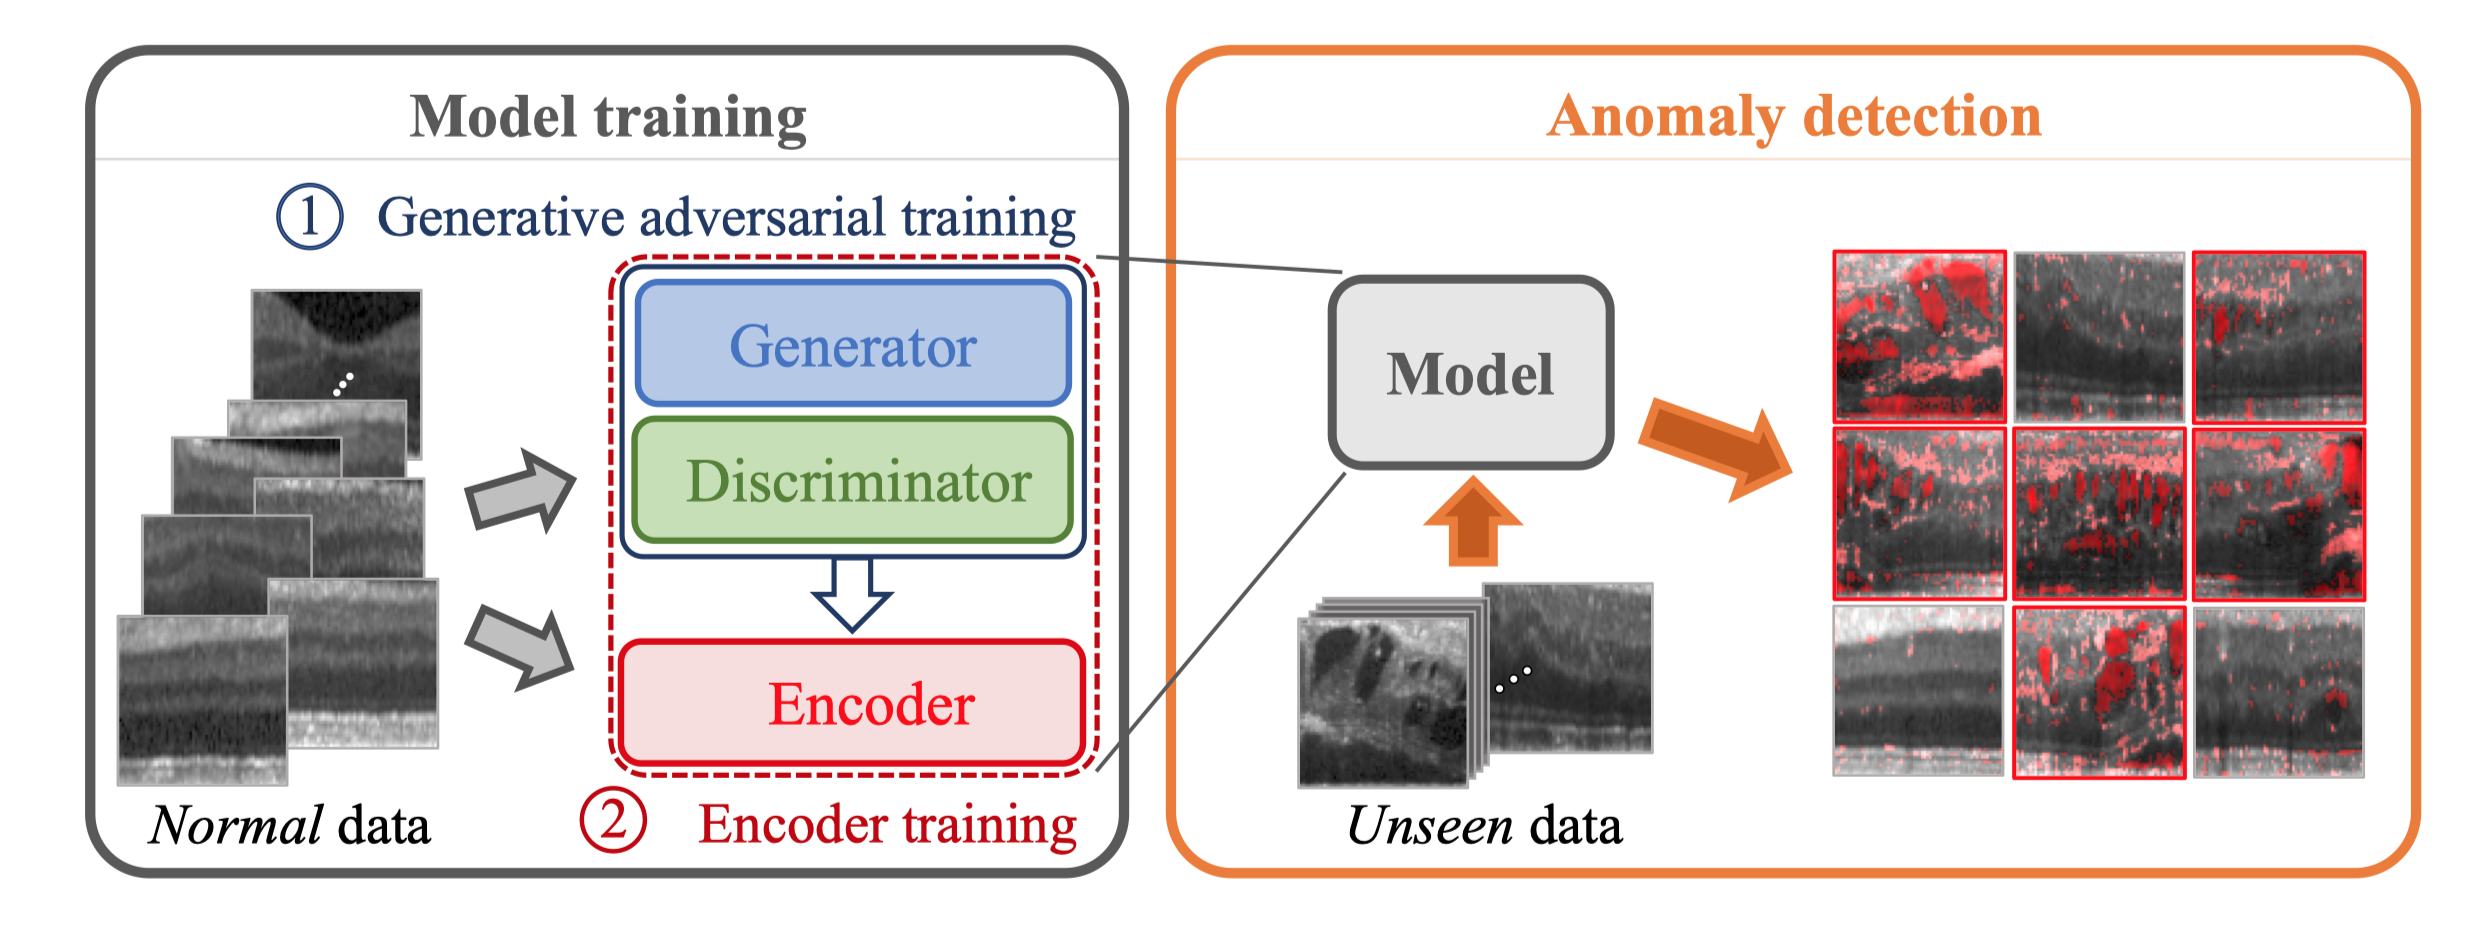
\includegraphics[width=.9\textwidth]{fanogan_framework}
	\caption{F-AnoGAN Framework Overview \cite{pub.1111824956}}
	\label{fig:fanogan_network}
\end{figure}

The first improvement is the change of the training style of the whole framework. In BiGAN approach,
encoder and generator is trained simultaneously to fool the discriminator. Hence discriminator is
modified to classify the pairs of noise (latent representation) and images instead of the single
image approach used in the GAN framework. Therefore it tries to distinguish samples from a joint
distribution which explained in section \ref{sec:bigan}. Including encoder to the adversarial setup
also introduces instability issues which ALAD Framework \cite{DBLP:journals/corr/abs-1812-02288}
tried to mitigate with additional discriminators that approaximate conditional entropy. (section
\ref{sec:alad_alice}). F-AnoGAN framework addresses this issue by seperating the training of the
encoder from the generator discriminator pair. The new framework can be seen in figure
\ref{fig:fanogan_training}. 
\begin{figure}[h!]
	\centering
	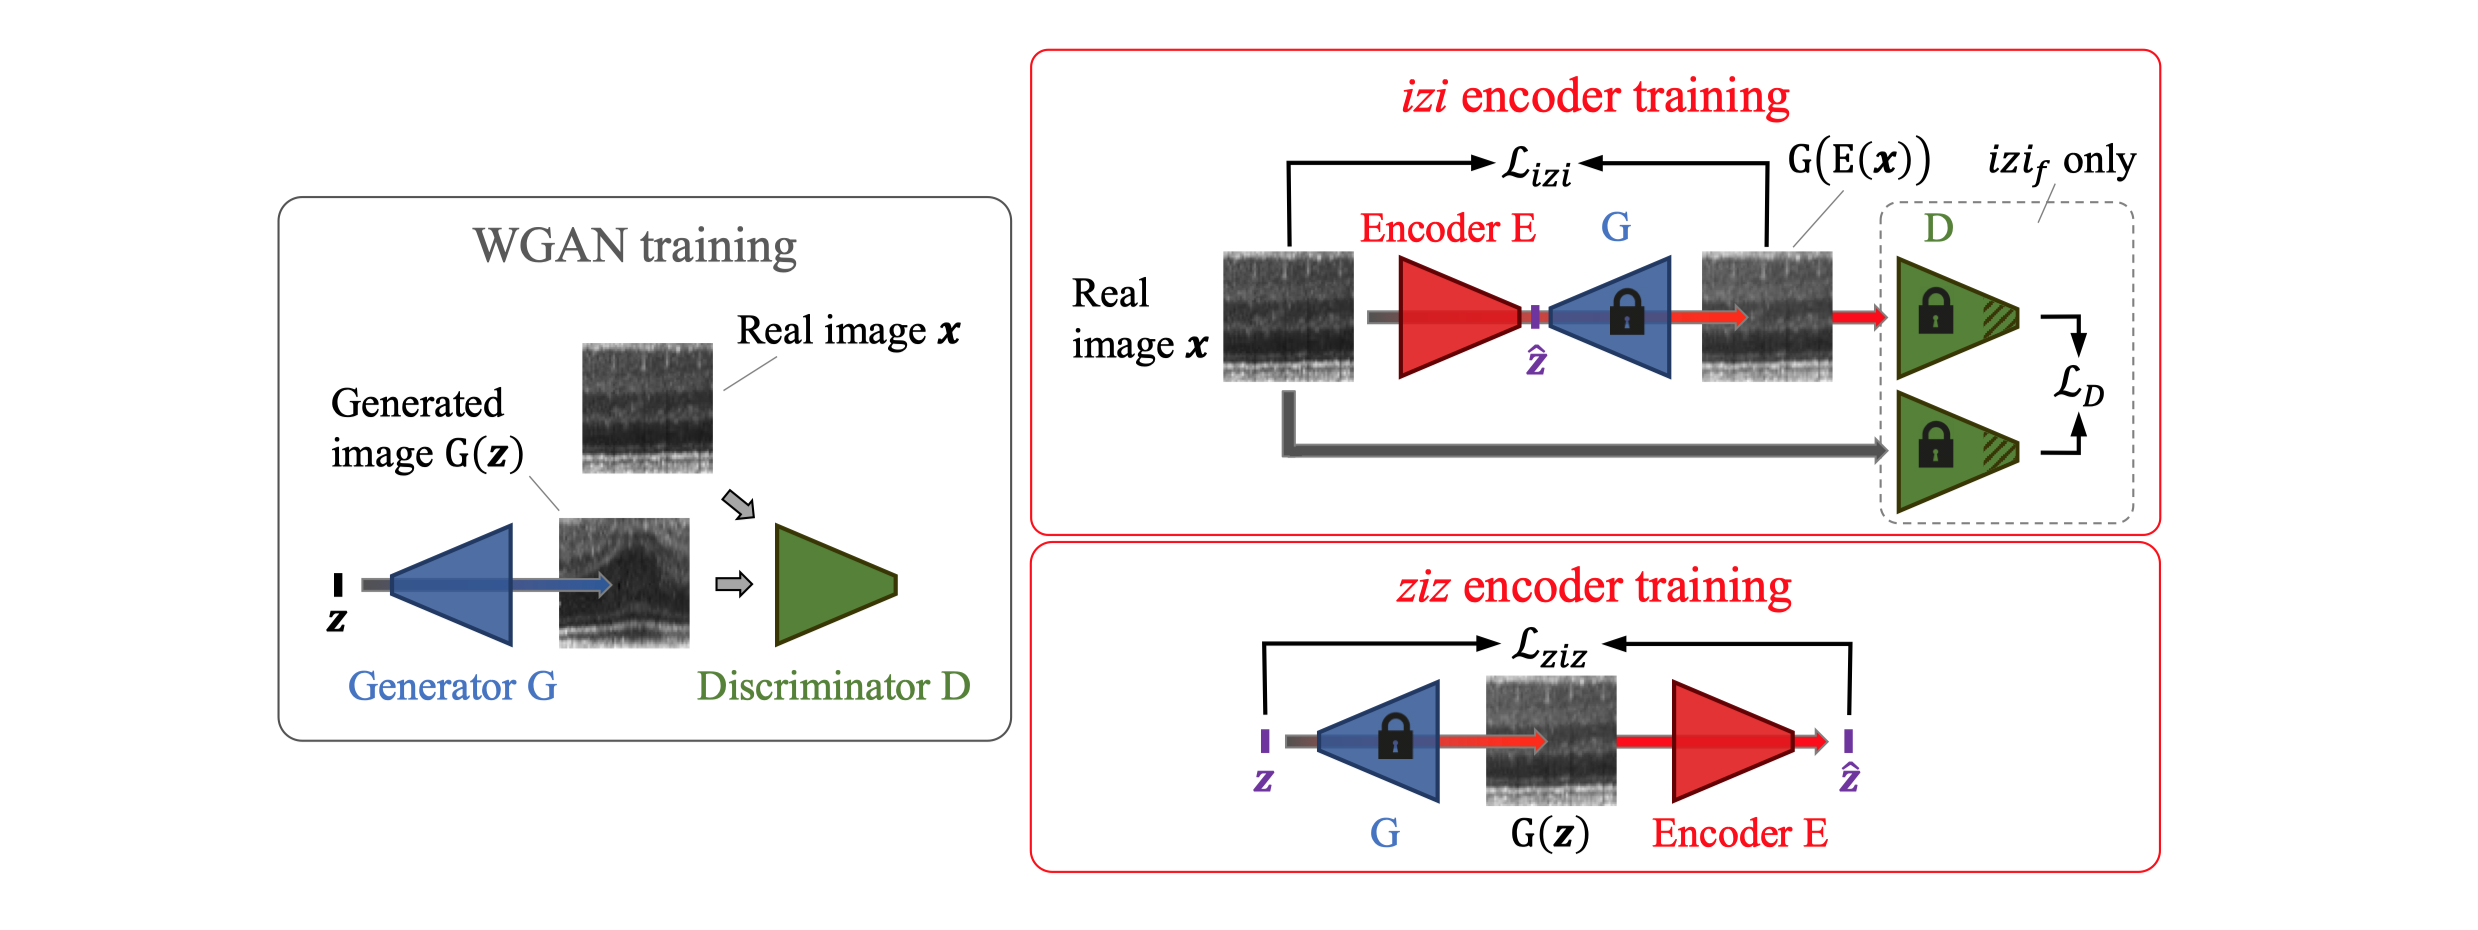
\includegraphics[width=.9\textwidth]{fanogan_training}
	\caption{F-AnoGAN Training Strategies \cite{pub.1111824956}}
	\label{fig:fanogan_training}
\end{figure}

This new training scheme comprises of the stages. In the first stage GAN framework is trained. The
objective function for the adversarial training is also replaced with the Wasserstein GAN's
objective function \cite{Arjovsky2017WassersteinG} 
% appendix explanation ?
although training of the GAN can be performed with any other framework's approach (including the
original GAN framework) according to the \cite{pub.1111824956}.

In the second stage, encoder network is trained using generator and discriminator with locked
weight. Two seperate pipelines are used to measure the performance of the encoder. These are izi
(image-noise-image) and ziz (noise-image-noise) respectively. 

\textbf{IZI Encoder Training}

$IZI$ method follows the standard autoencoder network approach. The generator network with fixed
weights acts as a decoder network. During the training, same image dataset used in the first stage
for training gan is mapped to a latent mapping $z$ by a trainable encoder and then reconstructed
using the fixed generator network. Training objective for this setup is to minimize MSE (Mean
Squared Error) based reconstruction error of the input image $x$ and the reconstructed image
$G(E(x))$. 
\begin{equation}
	\mathcal{L}_{i z i}(\mathbf{x})=\frac{1}{n}\|\mathbf{x}-G(E(\mathbf{x}))\|^{2}
\end{equation}

This approach has an important drawback regarding to latent representation. Since the distribution
of the latent representation of the input image is not known, the encoder is trained only using a
form of contextual loss which enforce the similarity only in the image space. Without the
insufficient information about the latent space, encoder may map images to a representations such
that the reconstructions are not convincing enough for the discriminator to evaluate as real.
\cite{pub.1111824956}. Therefore the framework suggests also including a latent space based loss
function derived from the feature layer of the discriminator to guide the encoder training. Improved
$izi_{f}$ training objective is defined below.
\begin{equation}
	\mathcal{L}_{i z i_{f}}(\mathbf{x})=\frac{1}{n} \cdot\|\mathbf{x}-G(E(\mathbf{x}))\|^{2}+\frac{\kappa}{n_{d}} \cdot\|f(\mathbf{x})-f(G(E(\mathbf{x})))\|^{2}
\end{equation}

where the $f(\cdot)$ represents the feature layer of the discriminator as a statistics, $n_{d}$ is
the dimensionality of the intermediate feature representation $f$ and $\kappa$ denotes the weighting
factor for the inclusion of the discriminator guidance.

\textbf{ZIZ Encoder Training}

Different from the $IZI$ method, this approach reverses the auto encoder setup and forms a decoder
encoder architecture. A random sampled noise from the z-space is mapped to the image space using the
fixed generator and then generated sample is encoded using the trainable encoder network. The loss
for the training is defined as the MSE based reconstruction of the noise which depicted in equation
below. 
\begin{equation}
	\mathcal{L}_{z i z}(\mathbf{z})=\frac{1}{d}\|\mathbf{z}-E(G(\mathbf{z}))\|^{2}
\end{equation}

The shortcoming of this approach is that even though the encoder is trained with a loss that will
enforce a similarity in latent space, encoder sees only images that are generated by the generator.
It doesn't see any image samples from the training dataset which affects the contextual similarity
of the reconstruction of learned latent space distribution. 
\begin{figure}[h!] \subfloat[Anomaly Score computation scheme for izi and $izi_f$ method]{
		\begin{minipage}[c][1\width]{0.5\textwidth}
			\centering
			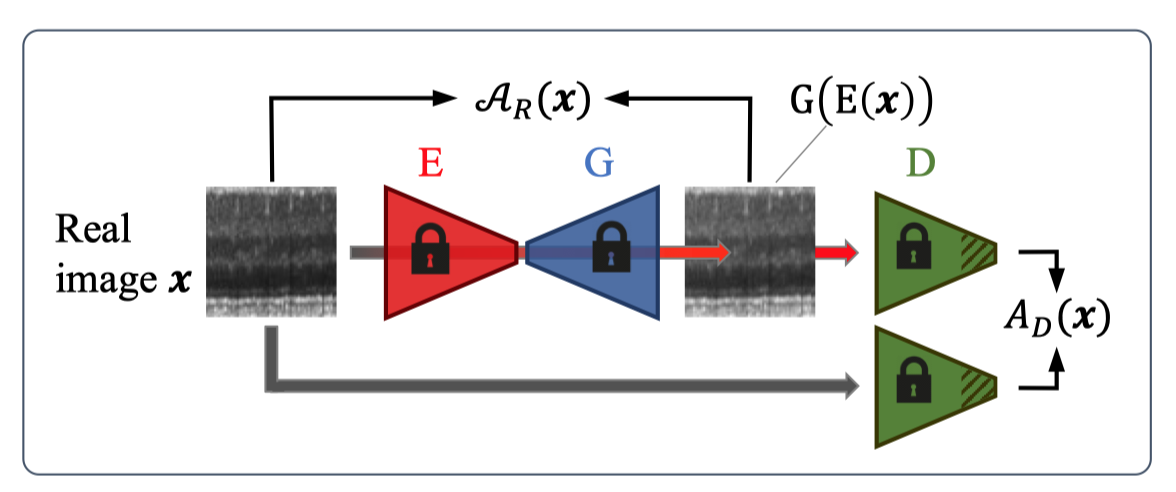
\includegraphics[width=1\textwidth]{fanogan_anomaly_1}
	\end{minipage}}
	\hfill 	
	\subfloat[Anomaly Score computation scheme for ziz architecture]{
		\begin{minipage}[c][1\width]{0.5\textwidth}
			\centering
			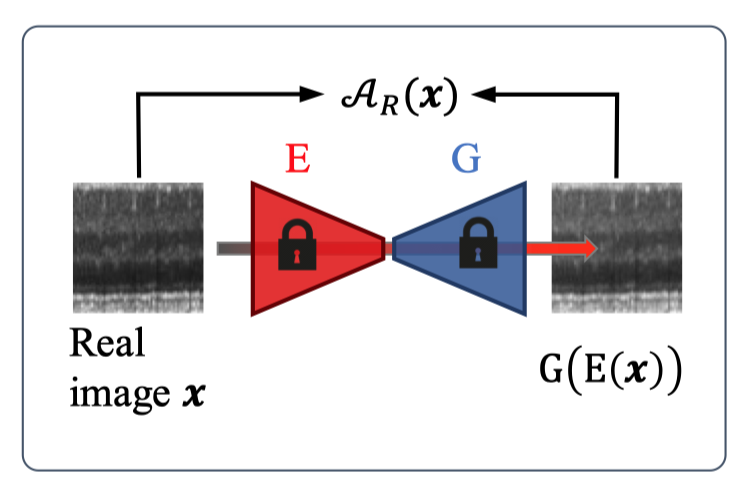
\includegraphics[width=0.6\textwidth]{fanogan_anomaly_2}
	\end{minipage}}
	\caption{Anomaly Score computations for both training methods \cite{pub.1111824956}}
	\label{fig:fanogan_anomaly_score}
\end{figure}

To calculate the anomaly score for inference, deviation of the query images from their
reconstructions are quantified. Figure \ref{fig:fanogan_anomaly_score} represents the anomaly score
computations for both training methods.

 $IZI_f$ method uses the same loss functions for the computation of the anomaly score. Anomaly score
 for image $x$ is defined as:
\begin{align}
	\mathcal{A}(\mathbf{x})&=\mathcal{A}_{R}(\mathbf{x})+\kappa \cdot \mathcal{A}_{D}(\mathbf{x}) \\[5pt]
	\mathcal{A}_{R}(\mathbf{x})&=\frac{1}{n} \cdot\|\mathbf{x}-G(E(\mathbf{x}))\|^{2} \\[5pt]
	\mathcal{A}_{D}(\mathbf{x})&=\frac{1}{n_{d}} \cdot\|f(\mathbf{x})-f(G(E(\mathbf{x})))\|^{2}
\end{align}

For $IZI$ and $ZIZ$ method, the computation of the anomaly score reduces down to
$\mathcal{A}_{R}(\mathbf{x})$ function only. Both training methods yields a similar anomaly score
computation for the anomalous samples. Since the models are trained with a dataset that doesn't
contain any anomalies, the query images that have anomalous regions results in poorer reconstruction
hence a higher anomaly score while the normal images produce a more similar reconstructions to the
original sample. 

The Significance of this framework is that it separates the training of the encoder from the
adversarial setting of the GAN's while preserving the inverse mapping functionality for the
inference. Chapter \ref{chap:arim} will explain its contribution to the proposed improved framework.

\section{Energy Based Generative Adversarial Networks}
\label{sec:ebgan}

Training a GAN framework perhaps the most sensitive part of working with them. There has been an
extensive amount of research to improve the stabilization of the adversarial training or perhaps
offer a new methodology. \cite{fm} and \cite{methods} offer number modifications to the original
adversarial training setup to improve the generation performance ,decrease the stabilization and
prevent issues such as mode collapse\footnotemark. \cite{Arjovsky2017WassersteinG} and
\cite{Gulrajani2017ImprovedTO} offers a new method to compute the loss and ways to stabilize it.
Mainly because of its adversarial setting, training of GAN frameworks will always be a topic of
interest. Energy based generative adversarial networks \cite{Zhao2016EnergybasedGA} offers a new
training method by redefining the loss functions and the functionality of the discriminator network.
This section will introduce the architecture and how it works.

\footnotetext{Mode collapse is the scenerio where generator learns enough information to fool the discriminator very early. It finds a generation that fools the discriminator and does not learn anything else from the discriminator. Because of that all the generated samples from the generator look the same, defeating the purpose of generating from the distribution of the data.\cite{methods}}

Energy based models measures the current state of the model by assigning a scalar predefined energy
as a degree of compatibility \cite{LeCun06atutorial}. Training energy based models consists of
mapping low energy outputs to the samples with the "correct" class, and mapping higher energy
outputs to the "incorrect" class. From the perspective of GANs, EBGAN model is trained to ouput
lower energy for the real data, while the generated data (fake images) outputs a higher energy. The
model architecture can be seen in figure \ref{fig:ebgan_model}.

\begin{figure}[h!]
	\centering
	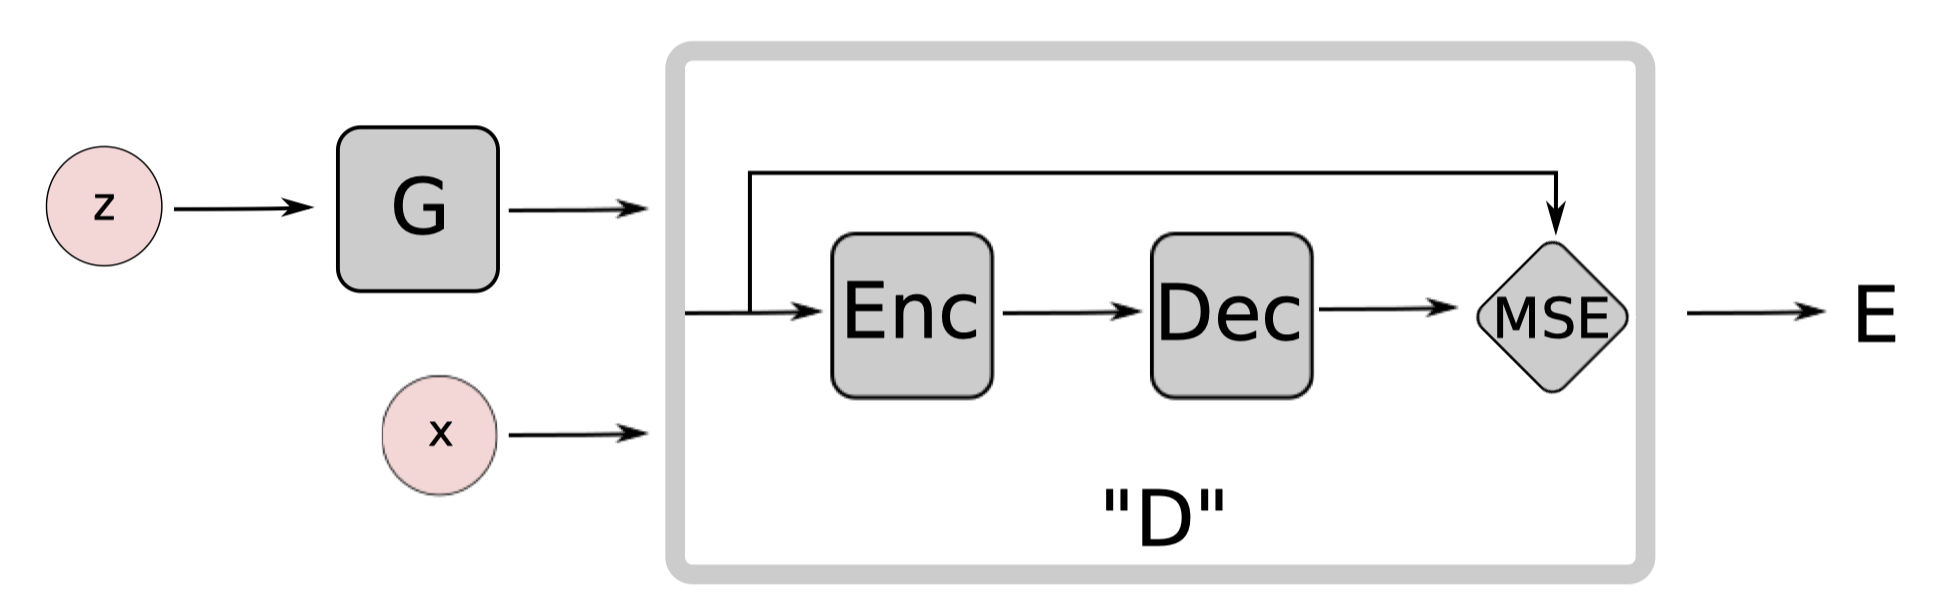
\includegraphics[width=1.0\textwidth]{ebgan_model}
	\caption{EBGAN Model Structure \cite{Zhao2016EnergybasedGA}}
	\label{fig:ebgan_model}
\end{figure}

The main structural difference of this framework from the other ones is that discriminator is
defined as an auto encoder network to provide the reconstruction of the inputs. The energy value
function is defined as the margin loss of the input and the reconstructed sample
\cite{Zhao2016EnergybasedGA} as a reconstruction error. 

Formally a margin is used to create an energy gap between the correct output and the incorrect
output. For data sample $x$, and a generated sample $G(z)$ with $z$ being sampled from a known
distribution $p_z$, The discriminator loss $\mathcal{L}_{D}$ and the generator loss
$\mathcal{L}_{G}$ are formally defined in equation \ref{eqn:ebgan_formal}.

\begin{equation}
\label{eqn:ebgan_formal}
\begin{aligned}D(x)&=\|\operatorname{Dec}(E n c(x))-x\|\\ \mathcal{L}_{D}(x, z) &=D(x)+[m-D(G(z))]^{+} \\ \mathcal{L}_{G}(z) &=D(G(z)) \end{aligned}
\end{equation}

where $D(x)$ is the reconstuction loss and  $[\cdot]^{+}=\max (0, \cdot)$. Minimizing
$\mathcal{L}_{G}$ with respect to the generator is similar to maximizing the second term of the
$\mathcal{L}_{D}$. Instead of calculating the probability of the input being real or fake,
discriminator is responsible for attaining the correct amount of energy to the input images. 

Using autoencoder network as a discriminator brings additional advantages to the training setting.
Rather than using a single target information to train the model, reconstruction based output offers
a more diverse targets for the discriminator \cite{Zhao2016EnergybasedGA}. One of the reasons of the
stabilization issues in the adversarial training is that discriminator might provide gradients not
useful enough for generator to improve the quality of the generated samples. Having a reconstruction
loss output might provide a better gradient in terms of different directions as opposed to binary
logistic loss. Another advantage is that even though they are trained with an adversarial setting,
autoencoder networks might prove useful to learn the underlying energy manifold of the data without
supervision or negative examples when they are trained using a proper regularization constraint.
This means that in this setting generated samples and input data are both used to model the
underlying energy manifold of the data. 

EBGAN framework argues that, the discriminator network is regularized by exposing generated samples
from the generator  which it should output higher reconstruction energies
\cite{Zhao2016EnergybasedGA}. The benefit of this regularization is that instead of a hand crafted
predefined one, the regularization term can also be trained along with the discriminator.
Adversarial training allows a direct connection between learning the energy function and producing
contradictive samples in that regard. 

EBGAN framework also adds additional penalty called pulling away term (PT) that run at a
representation level to prevent mode collapse depicted in equation \ref{eqn:ebgan_pt}.

\begin{equation}
\label{eqn:ebgan_pt}
	f_{P T}(S)=\frac{1}{N(N-1)} \sum_{i} \sum_{j \neq i}\left(\frac{S_{i}^{\top} S_{j}}{\left\|S_{i}\right\|\left\|S_{j}\right\|}\right)^{2}
\end{equation}

 $S$ is the feature output from the encoder for generated images. Pulling-away term measures the
 cosine similarity among all generated images features $S$ in a minibatch. If the mode collapses,
 the feature vectors will thereupon be similar, i.e. the angles are close to zero and the cosine
 will max-out. Therefore, it will add a high penalty if there are too similar.
 \cite{Zhao2016EnergybasedGA}
 
 

\endgroup
